% Template GRASS newsletter - Article
% Language: Latex
%

% Head
\graphicspath{{./images/}}

\title{Manuel de de\'butant du SIG Quantum pour le SIG GRASS}
\subtitle{}
\author{GRASS Development Team}

\maketitle

\section{INTRODUCTION AU SIG QUANTUM}

Ce Manuel est valide pour QGIS version 0.8 et plus (http://www.qgis.org)
\textbf{Lancez QGIS}, la premi\`ere fois cel\`a doit ressembler \`a Fig.~\ref{fig:qgis000}

%\setkeys{Gin}{width=1\textwidth}
\begin{figure}[htbp]
   \centering
   %name of your graphic, without the path AND in PNG (screnshots etc)/PDF (drawings) format:
   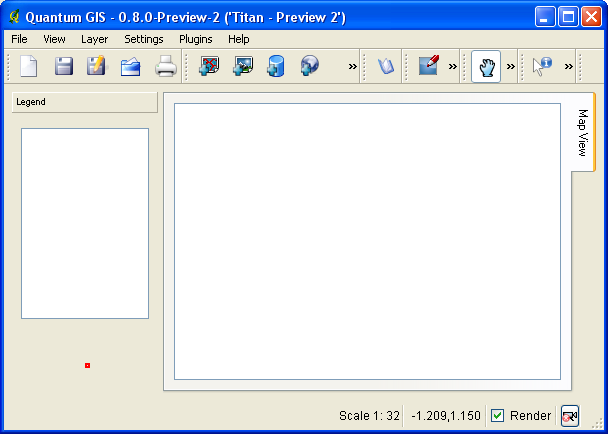
\includegraphics[scale=0.35]{qgis000.png}
   %caption of the figure
   \caption{}
   %label of the figure, which has to correspond to \ref{}:
   \label{fig:qgis000}
\end{figure}

Ouvrez quelques couches vectorielles venant des exemples de donn\'ees fournies avec QGIS Fig.~\ref{fig:qgis001}

%\setkeys{Gin}{width=1\textwidth}
\begin{figure}[htbp]
   \centering
   %name of your graphic, without the path AND in PNG (screnshots etc)/PDF (drawings) format:
   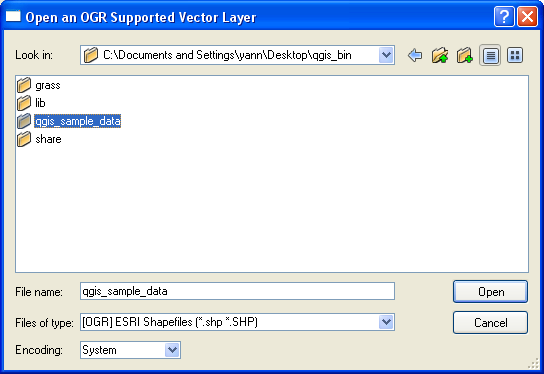
\includegraphics[scale=0.35]{qgis001.png}
   %caption of the figure
   \caption{}
   %label of the figure, which has to correspond to \ref{}:
   \label{fig:qgis001}
\end{figure}

S\'electionnez toutes les couches (Ctrl+a) Fig.~\ref{fig:qgis002}

%\setkeys{Gin}{width=1\textwidth}
\begin{figure}[htbp]
   \centering
   %name of your graphic, without the path AND in PNG (screnshots etc)/PDF (drawings) format:
   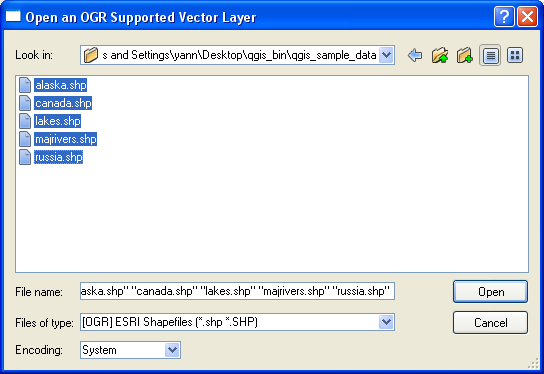
\includegraphics[scale=0.35]{qgis002.png}
   %caption of the figure
   \caption{}
   %label of the figure, which has to correspond to \ref{}:
   \label{fig:qgis002}
\end{figure}

Les couches affich\'ees devraient ressembler \`a cel\`a Fig.~\ref{fig:qgis003}

%\setkeys{Gin}{width=1\textwidth}
\begin{figure}[htbp]
   \centering
   %name of your graphic, without the path AND in PNG (screnshots etc)/PDF (drawings) format:
   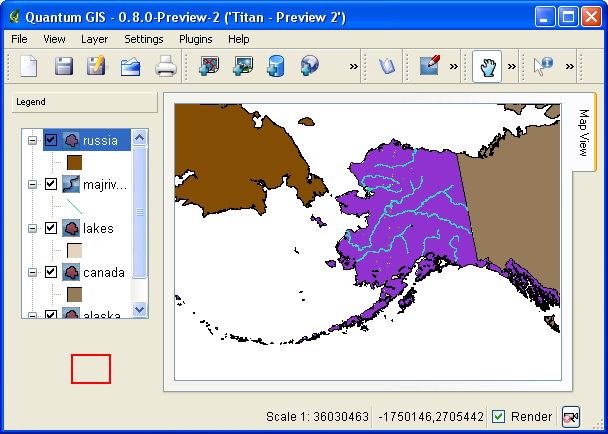
\includegraphics[scale=0.35]{qgis003.png}
   %caption of the figure
   \caption{}
   %label of the figure, which has to correspond to \ref{}:
   \label{fig:qgis003}
\end{figure}

Zoomez \`a l'\'etendue de toutes les couches ensemble... Fig.~\ref{fig:qgis004}

%\setkeys{Gin}{width=1\textwidth}
\begin{figure}[htbp]
   \centering
   %name of your graphic, without the path AND in PNG (screnshots etc)/PDF (drawings) format:
   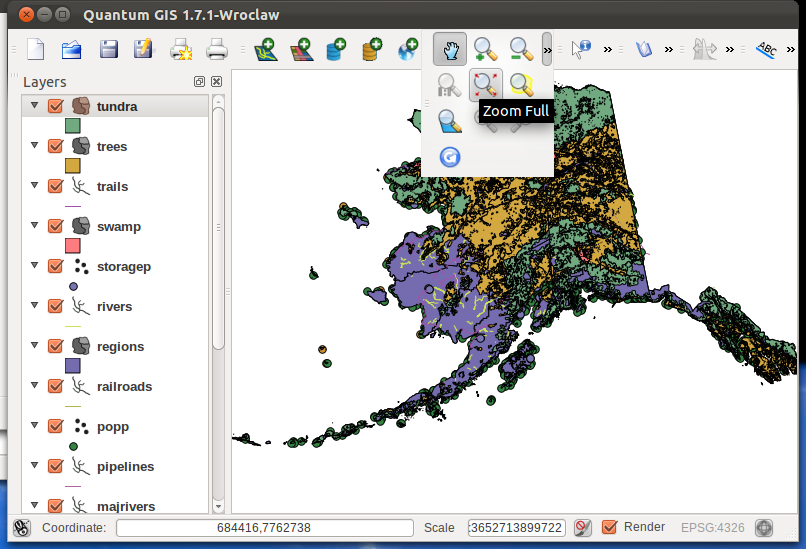
\includegraphics[scale=0.2]{qgis004.png}
   %caption of the figure
   \caption{}
   %label of the figure, which has to correspond to \ref{}:
   \label{fig:qgis004}
\end{figure}

R\'esultat apr\`es le zoom Fig.~\ref{fig:qgis005}

%\setkeys{Gin}{width=1\textwidth}
\begin{figure}[htbp]
   \centering
   %name of your graphic, without the path AND in PNG (screnshots etc)/PDF (drawings) format:
   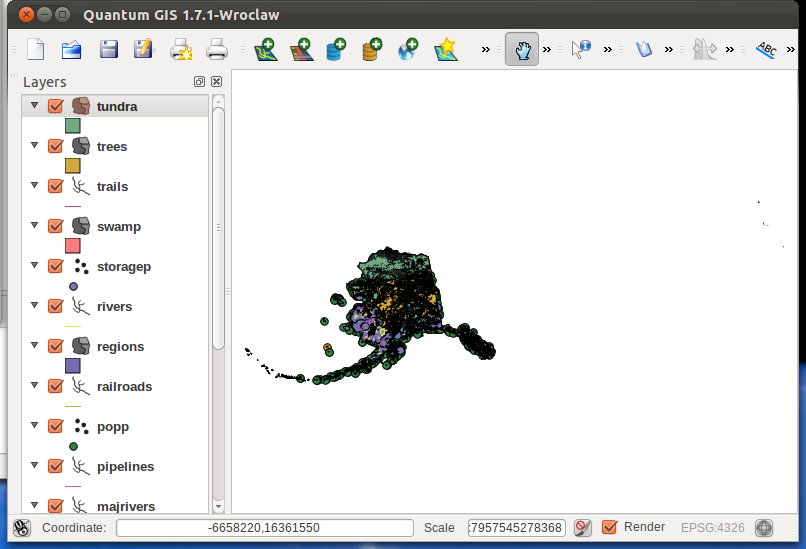
\includegraphics[scale=0.2]{qgis005.png}
   %caption of the figure
   \caption{}
   %label of the figure, which has to correspond to \ref{}:
   \label{fig:qgis005}
\end{figure}

Mettez la premi\`ere couche dans le cadre de survol Fig.~\ref{fig:qgis006}

%\setkeys{Gin}{width=1\textwidth}
\begin{figure}[htbp]
   \centering
   %name of your graphic, without the path AND in PNG (screnshots etc)/PDF (drawings) format:
   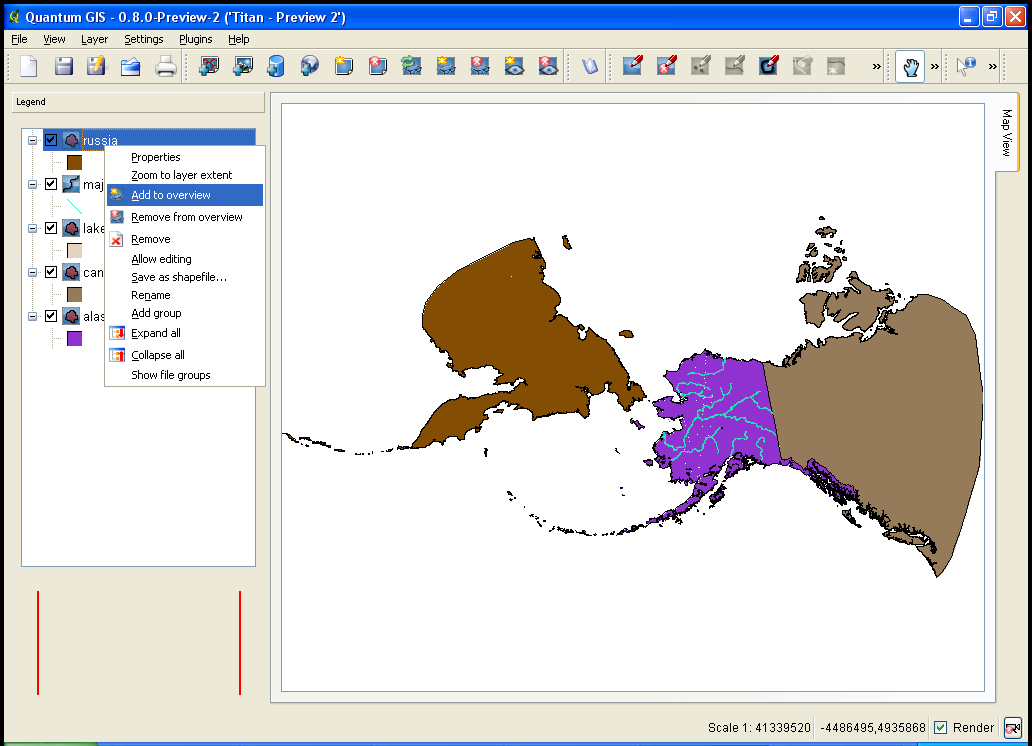
\includegraphics[scale=0.2]{qgis006.png}
   %caption of the figure
   \caption{}
   %label of the figure, which has to correspond to \ref{}:
   \label{fig:qgis006}
\end{figure}

R\'esultat... Fig.~\ref{fig:qgis007}

%\setkeys{Gin}{width=1\textwidth}
\begin{figure}[htbp]
   \centering
   %name of your graphic, without the path AND in PNG (screnshots etc)/PDF (drawings) format:
   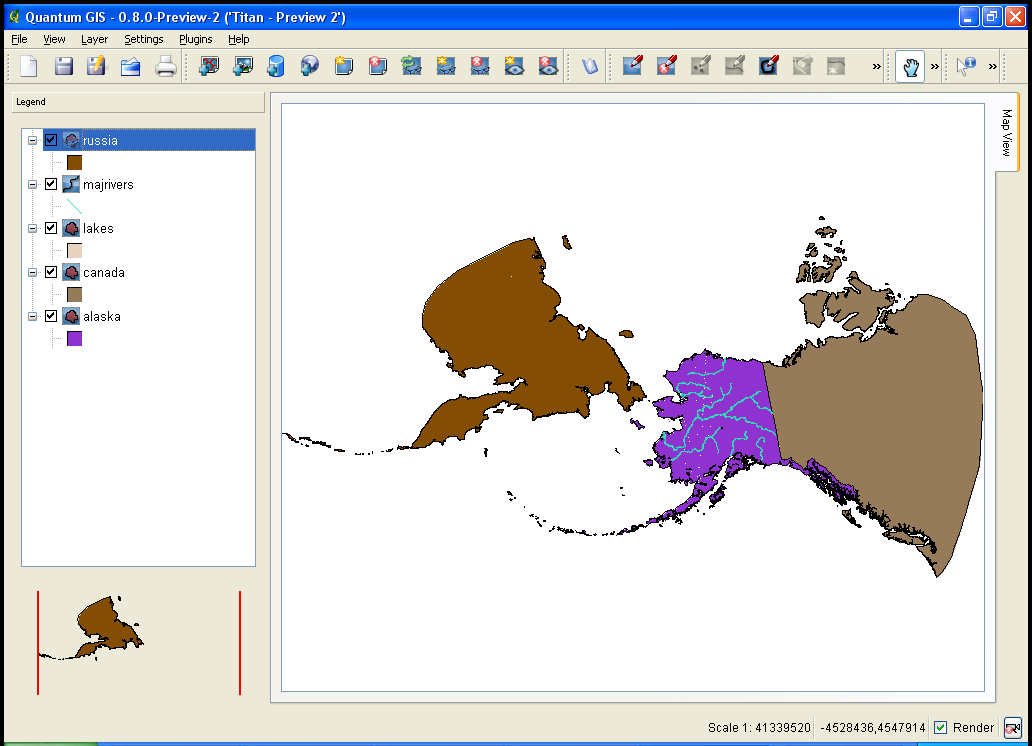
\includegraphics[scale=0.2]{qgis007.png}
   %caption of the figure
   \caption{}
   %label of the figure, which has to correspond to \ref{}:
   \label{fig:qgis007}
\end{figure}

Ouvrez le menu des plugins Fig.~\ref{fig:qgis008}

%\setkeys{Gin}{width=1\textwidth}
\begin{figure}[htbp]
   \centering
   %name of your graphic, without the path AND in PNG (screnshots etc)/PDF (drawings) format:
   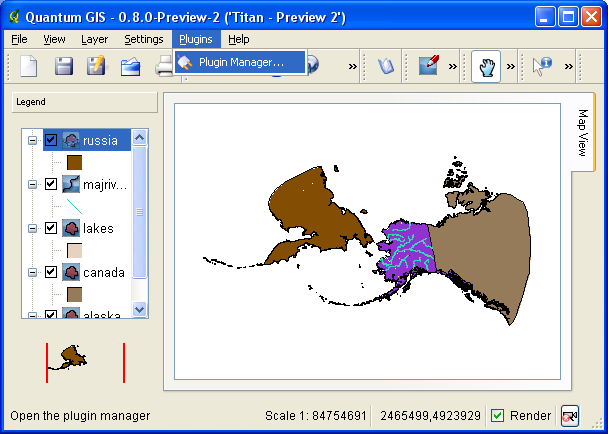
\includegraphics[scale=0.35]{qgis008.png}
   %caption of the figure
   \caption{}
   %label of the figure, which has to correspond to \ref{}:
   \label{fig:qgis008}
\end{figure}

Cel\`a devrait ressembler \`a la Fig.~\ref{fig:qgis009}

%\setkeys{Gin}{width=1\textwidth}
\begin{figure}[htbp]
   \centering
   %name of your graphic, without the path AND in PNG (screnshots etc)/PDF (drawings) format:
   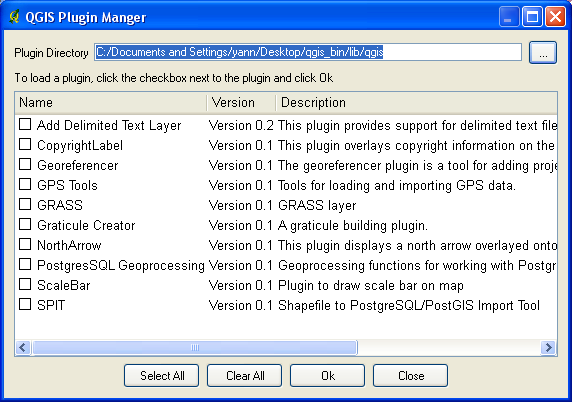
\includegraphics[scale=0.35]{qgis009.png}
   %caption of the figure
   \caption{}
   %label of the figure, which has to correspond to \ref{}:
   \label{fig:qgis009}
\end{figure}

S\'electionnez ces plugins Fig.~\ref{fig:qgis010}

%\setkeys{Gin}{width=1\textwidth}
\begin{figure}[htbp]
   \centering
   %name of your graphic, without the path AND in PNG (screnshots etc)/PDF (drawings) format:
   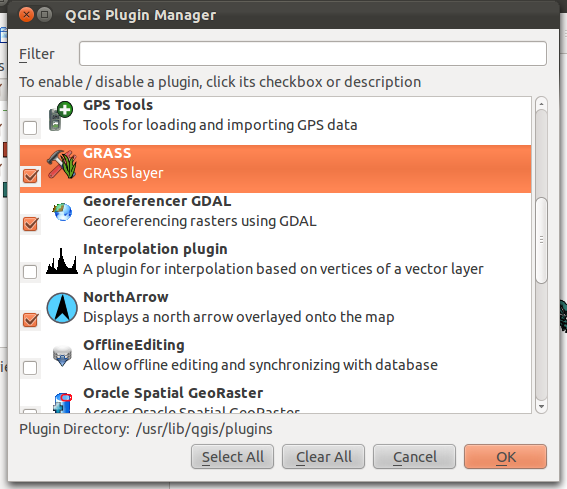
\includegraphics[scale=0.35]{qgis010.png}
   %caption of the figure
   \caption{}
   %label of the figure, which has to correspond to \ref{}:
   \label{fig:qgis010}
\end{figure}


De nouveaux menus sont apparus! Fig.~\ref{fig:qgis011}

%\setkeys{Gin}{width=1\textwidth}
\begin{figure}[htbp]
   \centering
   %name of your graphic, without the path AND in PNG (screnshots etc)/PDF (drawings) format:
   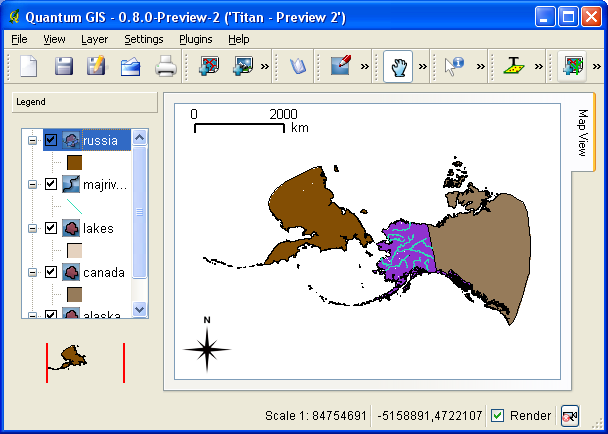
\includegraphics[scale=0.35]{qgis011.png}
   %caption of the figure
   \caption{}
   %label of the figure, which has to correspond to \ref{}:
   \label{fig:qgis011}
\end{figure}


En maximisant QGIS, plus d'ic\^ones apparaissent... Fig.~\ref{fig:qgis012}

%\setkeys{Gin}{width=1\textwidth}
\begin{figure}[htbp]
   \centering
   %name of your graphic, without the path AND in PNG (screnshots etc)/PDF (drawings) format:
   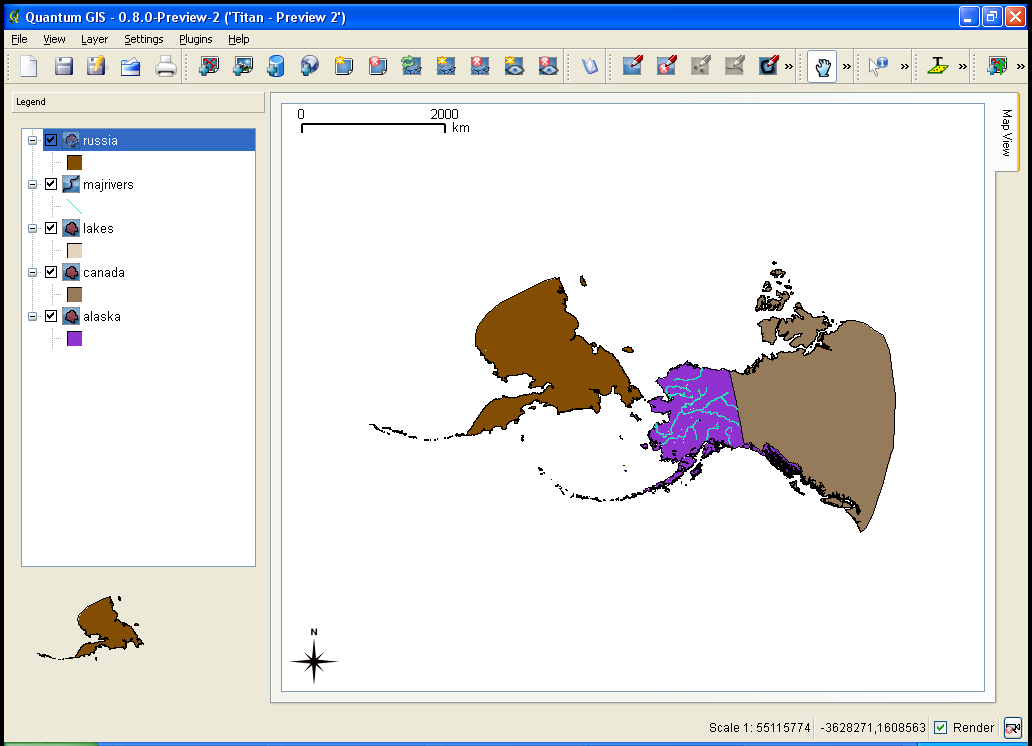
\includegraphics[scale=0.2]{qgis012.png}
   %caption of the figure
   \caption{}
   %label of the figure, which has to correspond to \ref{}:
   \label{fig:qgis012}
\end{figure}


Tirez les nouveaux menus en-dessous pour les faire coller au deuxi\`eme niveau de barre d'outil... Fig.~\ref{fig:qgis013}

%\setkeys{Gin}{width=1\textwidth}
\begin{figure}[htbp]
   \centering
   %name of your graphic, without the path AND in PNG (screnshots etc)/PDF (drawings) format:
   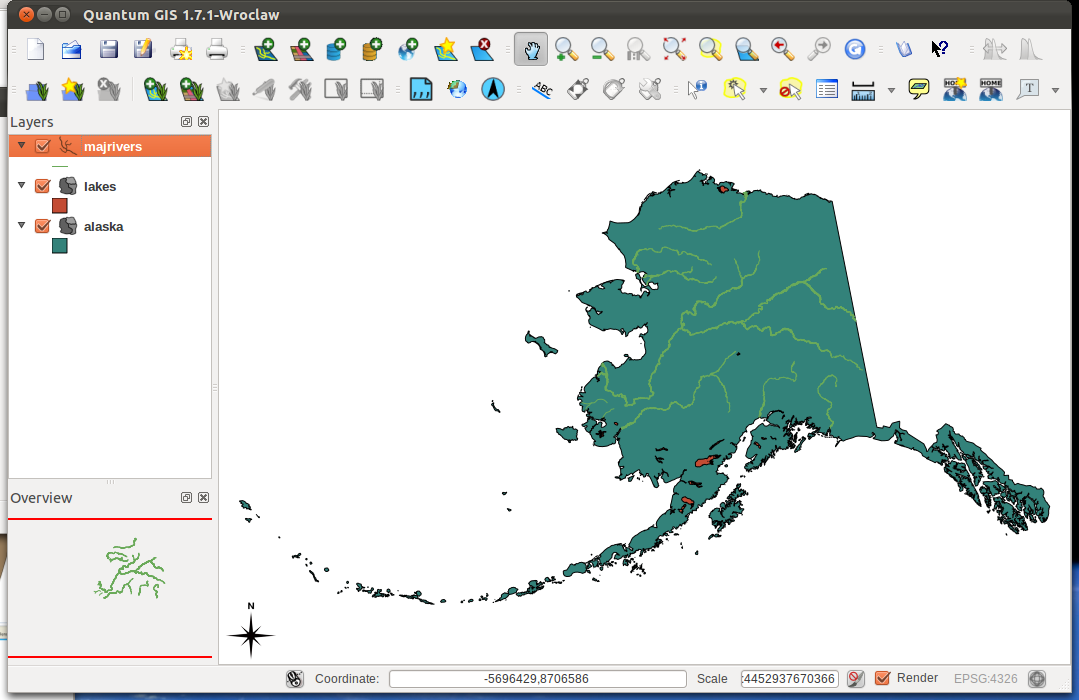
\includegraphics[scale=0.2]{qgis013.png}
   %caption of the figure
   \caption{}
   %label of the figure, which has to correspond to \ref{}:
   \label{fig:qgis013}
\end{figure}

\section{LE PLUGIN GRASS DANS LE SIG QUANTUM}

Ouvrez une couche raster GRASS en cliquant sur le second bouton \`a partir de la gauche Fig.~\ref{fig:qgis014}

%\setkeys{Gin}{width=1\textwidth}
\begin{figure}[htbp]
   \centering
   %name of your graphic, without the path AND in PNG (screnshots etc)/PDF (drawings) format:
   
\includegraphics[scale=0.45]{qgis014.png}
   %caption of the figure
   \caption{}
   %label of the figure, which has to correspond to \ref{}:
   \label{fig:qgis014}
\end{figure}

Ceci est le menu contextuel s'ouvrant, s\'electionnez le nom de carte ``elevation.10m'' Fig.~\ref{fig:qgis015}

%\setkeys{Gin}{width=1\textwidth}
\begin{figure}[htbp]
   \centering
   %name of your graphic, without the path AND in PNG (screnshots etc)/PDF (drawings) format:
   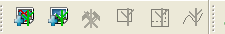
\includegraphics[scale=0.85]{qgis015.png}
   %caption of the figure
   \caption{}
   %label of the figure, which has to correspond to \ref{}:
   \label{fig:qgis015}
\end{figure}
 

Ceci est le r\'esultat du chargement de la couche raster de GRASS Fig.~\ref{fig:qgis016}

%\setkeys{Gin}{width=1\textwidth}
\begin{figure}[htbp]
   \centering
   %name of your graphic, without the path AND in PNG (screnshots etc)/PDF (drawings) format:
   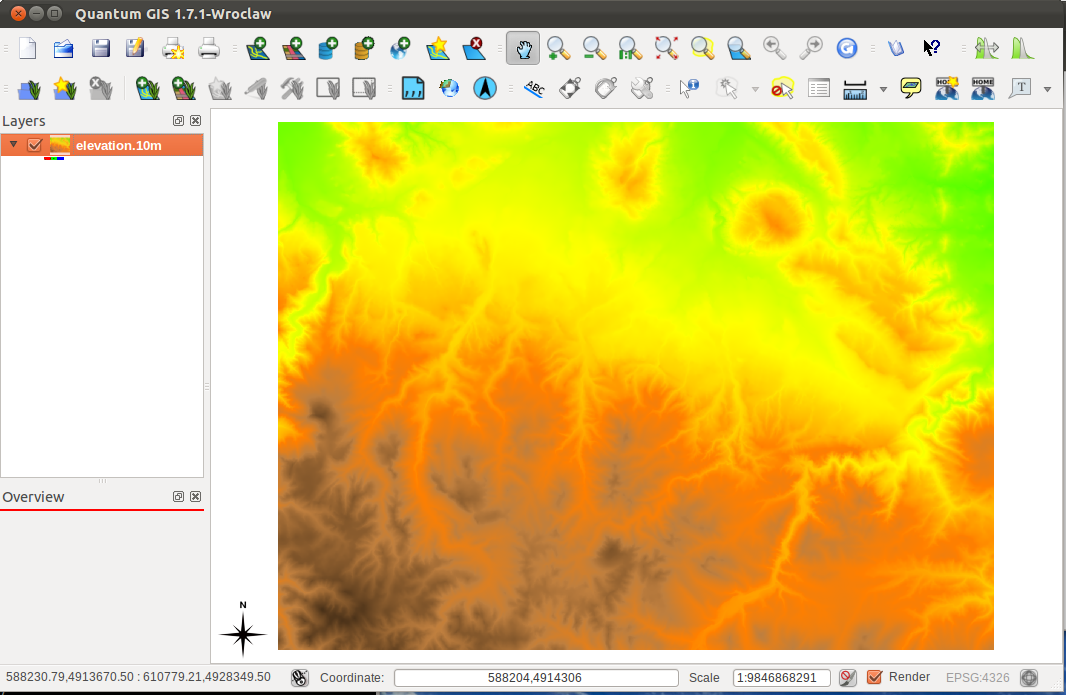
\includegraphics[scale=0.2]{qgis016.png}
   %caption of the figure
   \caption{}
   %label of the figure, which has to correspond to \ref{}:
   \label{fig:qgis016}
\end{figure}

De la m\^eme mani\`ere avec d'autres types de donn\'ees, ajoutez cette couche dans le cadre de survol Fig.~\ref{fig:qgis017}

%\setkeys{Gin}{width=1\textwidth}
\begin{figure}[htbp]
   \centering
   %name of your graphic, without the path AND in PNG (screnshots etc)/PDF (drawings) format:
   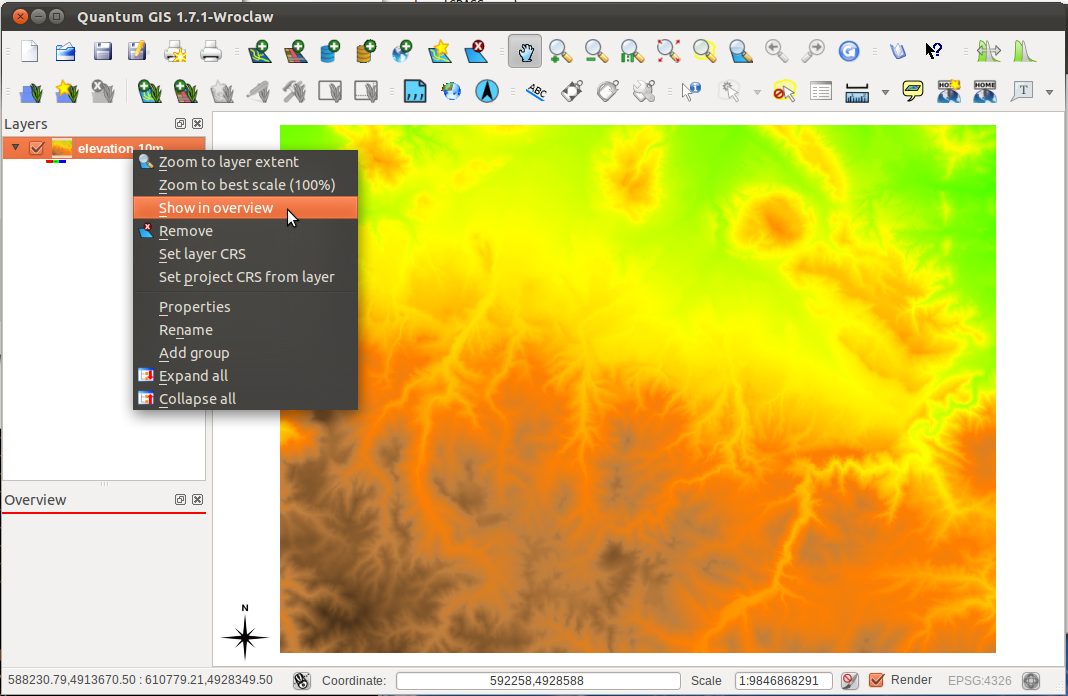
\includegraphics[scale=0.2]{qgis017.png}
   %caption of the figure
   \caption{}
   %label of the figure, which has to correspond to \ref{}:
   \label{fig:qgis0017}
\end{figure}

R\'esultat Fig.~\ref{fig:qgis018}

%\setkeys{Gin}{width=1\textwidth}
\begin{figure}[htbp]
   \centering
   %name of your graphic, without the path AND in PNG (screnshots etc)/PDF (drawings) format:
   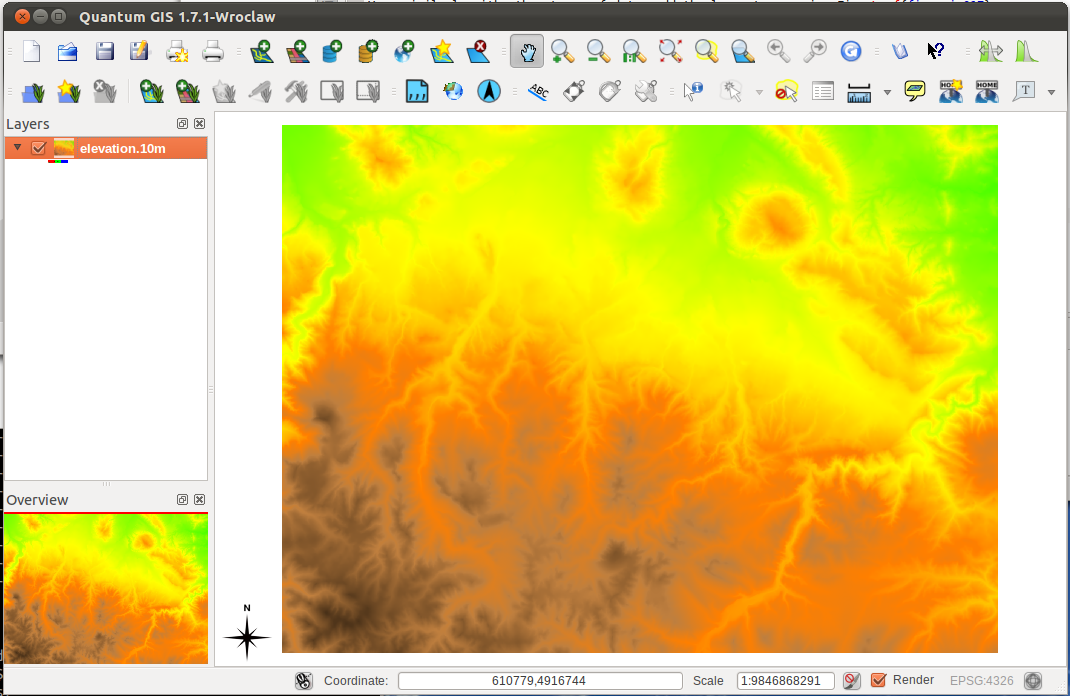
\includegraphics[scale=0.2]{qgis018.png}
   %caption of the figure
   \caption{}
   %label of the figure, which has to correspond to \ref{}:
   \label{fig:qgis018}
\end{figure}

Ajoutez une couche vectorielle de GRASS en s\'electionnant la premi\`ere ic\^one\`a partir de la gauche Fig.~\ref{fig:qgis019}

%\setkeys{Gin}{width=1\textwidth}
\begin{figure}[htbp]
   \centering
   %name of your graphic, without the path AND in PNG (screnshots etc)/PDF (drawings) format:
   
\includegraphics[scale=0.75]{qgis019.png}
   %caption of the figure
   \caption{}
   %label of the figure, which has to correspond to \ref{}:
   \label{fig:qgis019}
\end{figure}

Voici le menu contextuel qui s'ouvre, s\'electionnez la carte ayant le nom ``streams'' et sa couche de donn\'ees ``1\_Line'' Fig.~\ref{fig:qgis020}

%\setkeys{Gin}{width=1\textwidth}
\begin{figure}[htbp]
   \centering
   %name of your graphic, without the path AND in PNG (screnshots etc)/PDF (drawings) format:
   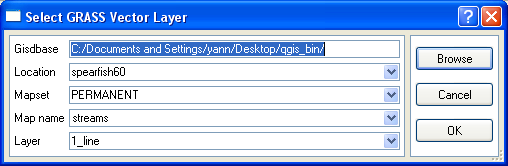
\includegraphics[scale=0.45]{qgis020.png}
   %caption of the figure
   \caption{}
   %label of the figure, which has to correspond to \ref{}:
   \label{fig:qgis020}
\end{figure}

Ceci est la couche vectorielle ``streams'', ouvrez les propri\'et\'es en cliquant sur le bouton droit sur le nom Fig.~\ref{fig:qgis021}

%\setkeys{Gin}{width=1\textwidth}
\begin{figure}[htbp]
   \centering
   %name of your graphic, without the path AND in PNG (screnshots etc)/PDF (drawings) format:
   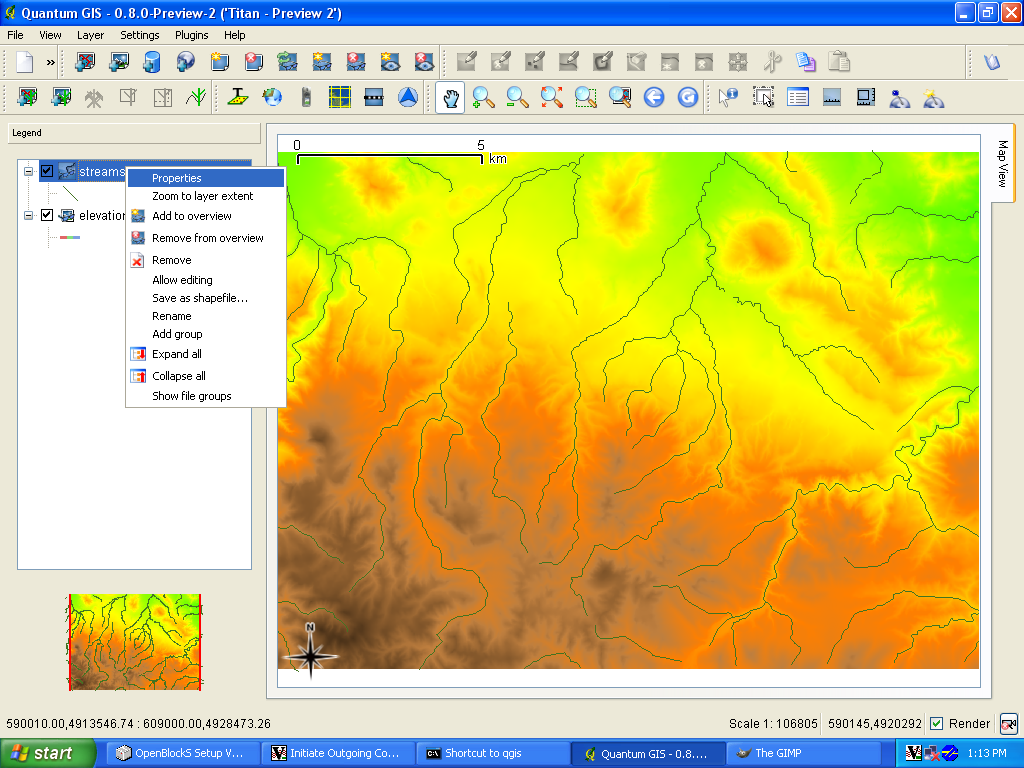
\includegraphics[scale=0.2]{qgis021.png}
   %caption of the figure
   \caption{}
   %label of the figure, which has to correspond to \ref{}:
   \label{fig:qgis021}
\end{figure}

La bo\^ite de propri\'et\'es ressemble \`a cel\`a, s\'electionnez le bouton ``fill color'' pour ouvrir une bo\^ite d'outils de s\'election de couleurs. Changez la couleur en un bleu commun et validez Fig.~\ref{fig:qgis022} Fig.~\ref{fig:qgis023}

%\setkeys{Gin}{width=1\textwidth}
\begin{figure}[htbp]
   \centering
   %name of your graphic, without the path AND in PNG (screnshots etc)/PDF (drawings) format:
   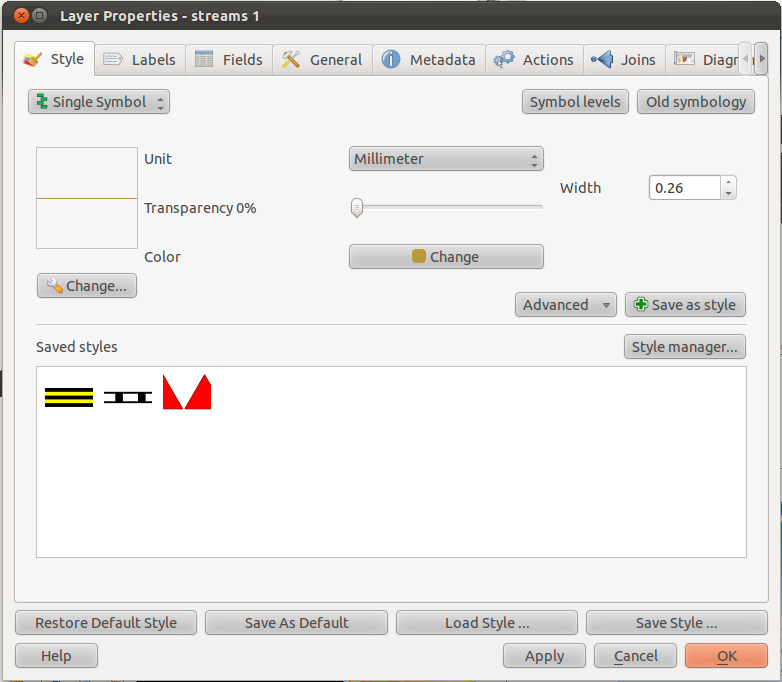
\includegraphics[scale=0.35]{qgis022.png}
   %caption of the figure
   \caption{}
   %label of the figure, which has to correspond to \ref{}:
   \label{fig:qgis022}
\end{figure}

%\setkeys{Gin}{width=1\textwidth}
\begin{figure}[htbp]
   \centering
   %name of your graphic, without the path AND in PNG (screnshots etc)/PDF (drawings) format:
   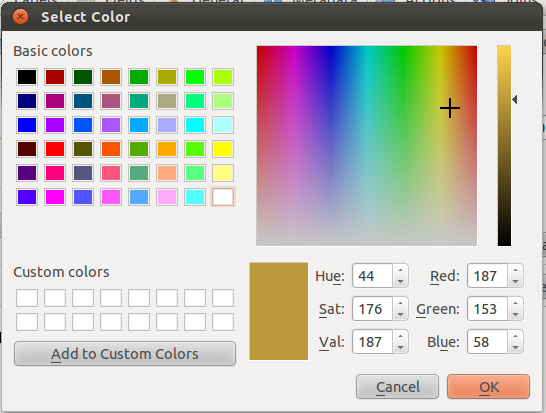
\includegraphics[scale=0.35]{qgis023.png}
   %caption of the figure
   \caption{}
   %label of the figure, which has to correspond to \ref{}:
   \label{fig:qgis023}
\end{figure}

S\'electionnez le premier bouton sur la droite pour commencer le module d'\'edition de vecteurs de GRASS Fig.~\ref{fig:qgis024}

%\setkeys{Gin}{width=1\textwidth}
\begin{figure}[htbp]
   \centering
   %name of your graphic, without the path AND in PNG (screnshots etc)/PDF (drawings) format:
   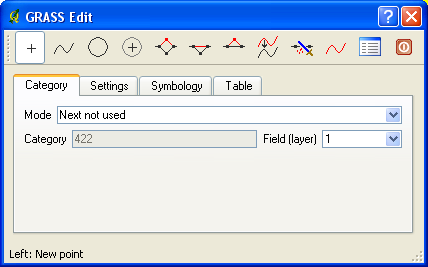
\includegraphics[scale=0.4]{qgis024.png}
   %caption of the figure
   \caption{}
   %label of the figure, which has to correspond to \ref{}:
   \label{fig:qgis024}
\end{figure}

La bo\^ite de dialogue de l'\'editeur de vecteurs de GRASS peut seulement \^etre ouverte si une couche vectorielle est s\'electionn\'ee dans la fen\^etre principale de QGIS Fig.~\ref{fig:qgis025}

%\setkeys{Gin}{width=1\textwidth}
\begin{figure}[htbp]
   \centering
   %name of your graphic, without the path AND in PNG (screnshots etc)/PDF (drawings) format:
   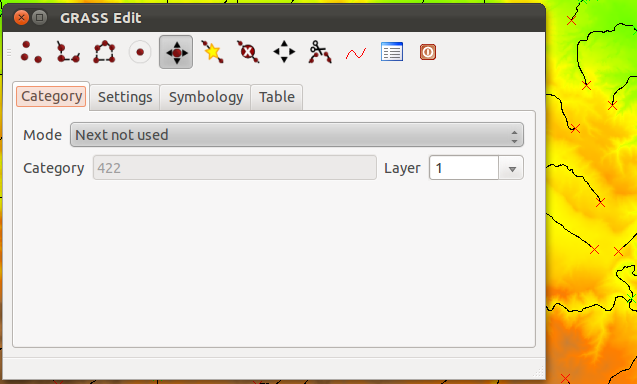
\includegraphics[scale=0.35]{qgis025.png}
   %caption of the figure
   \caption{}
   %label of the figure, which has to correspond to \ref{}:
   \label{fig:qgis025}
\end{figure}

S\'electionnez le bouton ``moving vertex'' (5\`eme de la gauche) et bougez la croix rouge sur la carte Fig.~\ref{fig:qgis026}

%\setkeys{Gin}{width=1\textwidth}
\begin{figure}[htbp]
   \centering
   %name of your graphic, without the path AND in PNG (screnshots etc)/PDF (drawings) format:
   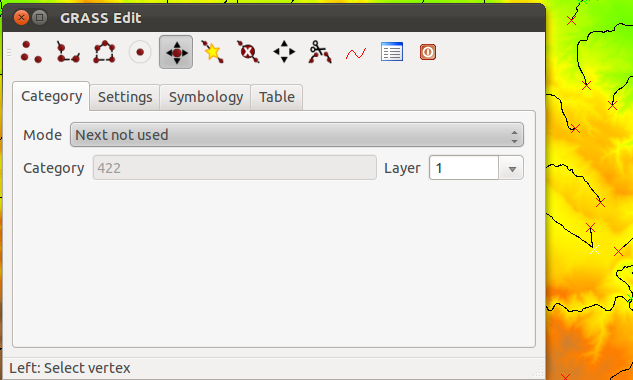
\includegraphics[scale=0.35]{qgis026.png}
   %caption of the figure
   \caption{}
   %label of the figure, which has to correspond to \ref{}:
   \label{fig:qgis026}
\end{figure}

Le r\'esultat devrait ressembler \`a ceci (Fig.~\ref{fig:qgis026}). Le dernier bouton de la barre d'outils va enregistrer les modifications effectu\'ees sur la couche vectorielle et la reconstruire Fig.~\ref{fig:qgis027}

%\setkeys{Gin}{width=1\textwidth}
\begin{figure}[htbp]
   \centering
   %name of your graphic, without the path AND in PNG (screnshots etc)/PDF (drawings) format:
   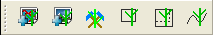
\includegraphics[scale=0.75]{qgis027.png}
   %caption of the figure
   \caption{}
   %label of the figure, which has to correspond to \ref{}:
   \label{fig:qgis027}
\end{figure}

Dans le terminal de lancement, l'enregistrement des changements apparaissent Fig.~\ref{fig:qgis028}

%\setkeys{Gin}{width=1\textwidth}
\begin{figure}[htbp]
   \centering
   %name of your graphic, without the path AND in PNG (screnshots etc)/PDF (drawings) format:
   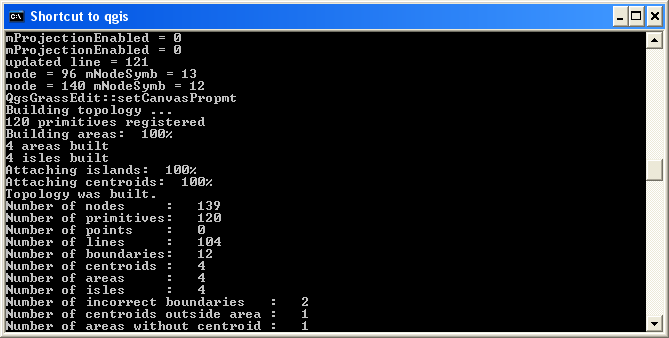
\includegraphics[scale=0.35]{qgis028.png}
   %caption of the figure
   \caption{}
   %label of the figure, which has to correspond to \ref{}:
   \label{fig:qgis028}
\end{figure}

Mettez en place l'environnement du plugin GRASS pour le traitement de donn\'ees... Fig.~\ref{fig:qgis029}

%\setkeys{Gin}{width=1\textwidth}
\begin{figure}[htbp]
   \centering
   %name of your graphic, without the path AND in PNG (screnshots etc)/PDF (drawings) format:
   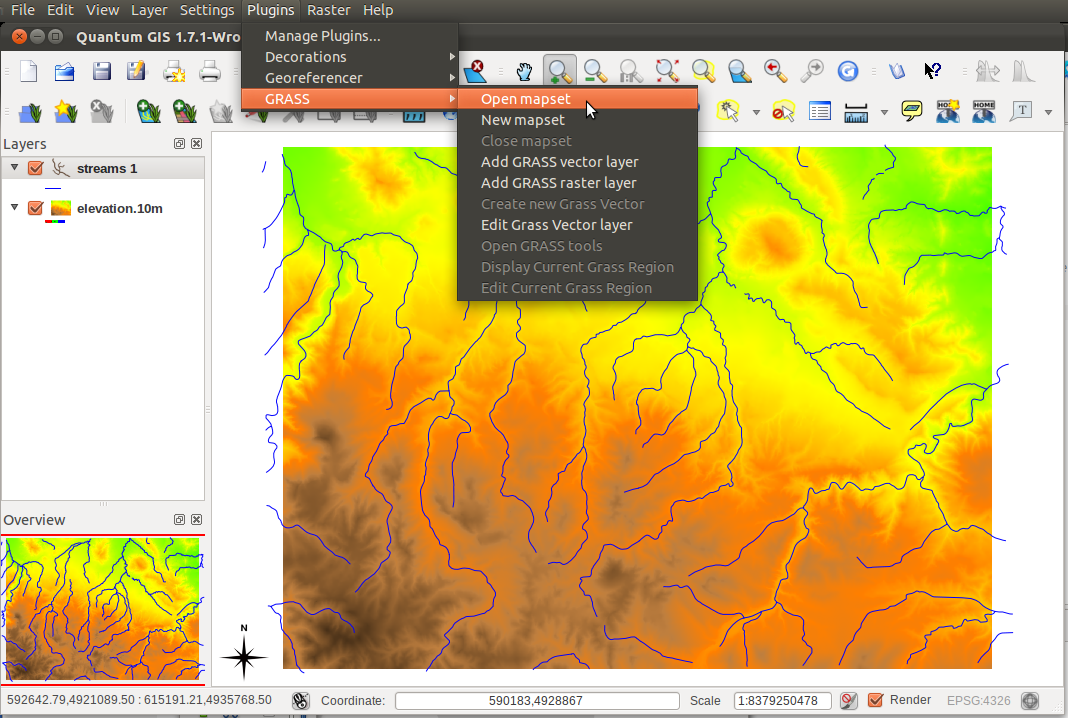
\includegraphics[scale=0.35]{qgis029.png}
   %caption of the figure
   \caption{}
   %label of the figure, which has to correspond to \ref{}:
   \label{fig:qgis029}
\end{figure}

Suivant ceci, s\'electionnez la 3\`eme ic\^one de gauche sur la barre d'outil GRASS. Cel\`a ouvrira l'outil de traitement de donn\'ees comme vu plus ou moins dans les 3 prochaines pages. Cet outil GRASS est une repr\'esentation mince des capacit\'es de GRASS, mais il va suffir aux besoins de cette introduction. Il est fournit avec un navigateur de jeu de cartes GRASS. Il agit aussi en temps qu'interface de gestion de donn\'ees. Fig.~\ref{fig:qgis030}

%\setkeys{Gin}{width=1\textwidth}
\begin{figure}[htbp]
   \centering
   %name of your graphic, without the path AND in PNG (screnshots etc)/PDF (drawings) format:
   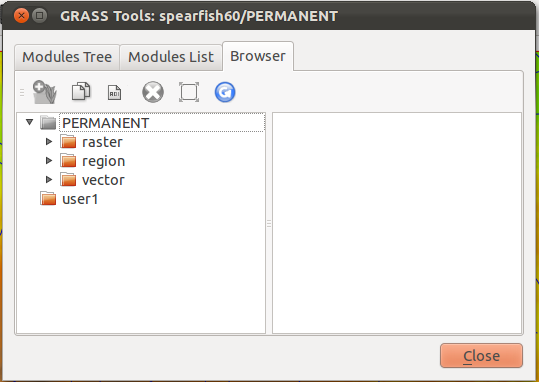
\includegraphics[scale=0.4]{qgis030.png}
   %caption of the figure
   \caption{}
   %label of the figure, which has to correspond to \ref{}:
   \label{fig:qgis030}
\end{figure}

Le navigateur a la capacit\'e d'ouvrir les informations d'en-t\^ete et de m\'eta-donn\'ees contenues dans les couches s\'electionn\'ees Fig.~\ref{fig:qgis031}

%\setkeys{Gin}{width=1\textwidth}
\begin{figure}[htbp]
   \centering
   %name of your graphic, without the path AND in PNG (screnshots etc)/PDF (drawings) format:
   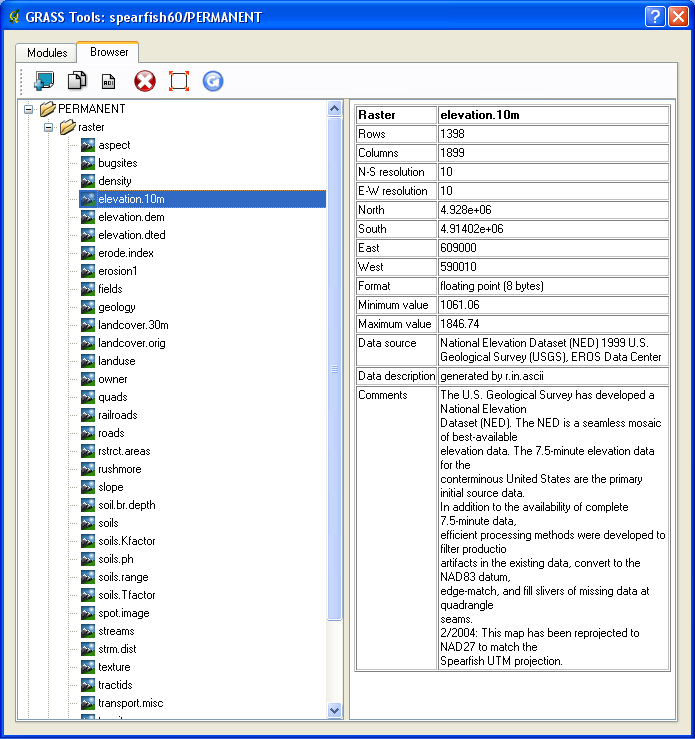
\includegraphics[scale=0.3]{qgis031.png}
   %caption of the figure
   \caption{}
   %label of the figure, which has to correspond to \ref{}:
   \label{fig:qgis031}
\end{figure}

Les modules GRASS disponibles sont list\'es dans les deux prochaines pages. Plus de modules sont int\'egr\'es tous les jours, le nombre actuel de modules de GRASS d\'epasse les 400, vous pouvez voir qu'il y a toujours du travail \`a faire, et que la communaut\'e de volontaires y travaillent Fig.~\ref{fig:qgis032} Fig.~\ref{fig:qgis033}

%\setkeys{Gin}{width=1\textwidth}
\begin{figure}[htbp]
   \centering
   %name of your graphic, without the path AND in PNG (screnshots etc)/PDF (drawings) format:
   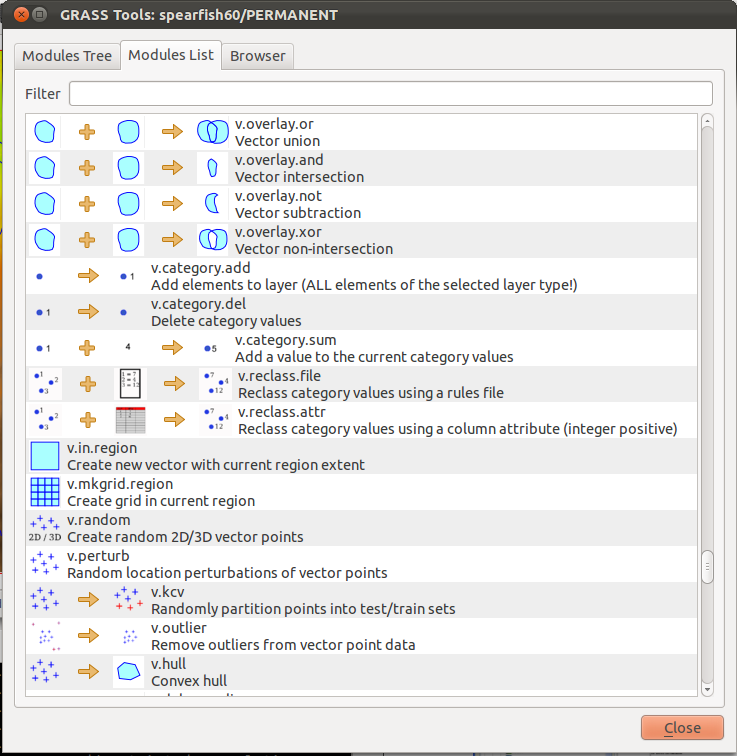
\includegraphics[scale=0.4]{qgis032.png}
   %caption of the figure
   \caption{}
   %label of the figure, which has to correspond to \ref{}:
   \label{fig:qgis032}
\end{figure}

%\setkeys{Gin}{width=1\textwidth}
\begin{figure}[htbp]
   \centering
   %name of your graphic, without the path AND in PNG (screnshots etc)/PDF (drawings) format:
   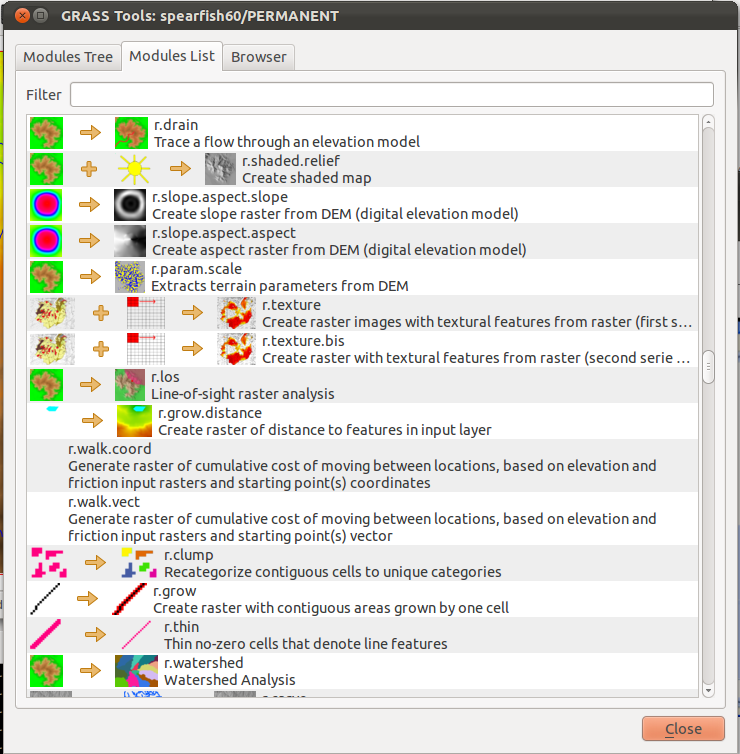
\includegraphics[scale=0.4]{qgis033.png}
   %caption of the figure
   \caption{}
   %label of the figure, which has to correspond to \ref{}:
   \label{fig:qgis033}
\end{figure}

\subsection{TRAITEMENT DE DONNEES AVEC LE PLUGIN GRASS}

Cr\'eons quelques buffers (zones tampon)... S\'electionnez ``buffering of vectors'' dans la liste des modules. Cel\`a devrait ressembler \`a ceci. Choisissez ue taille de zone tampon de 500 m\`etres Fig.~\ref{fig:qgis034}

%\setkeys{Gin}{width=1\textwidth}
\begin{figure}[htbp]
   \centering
   %name of your graphic, without the path AND in PNG (screnshots etc)/PDF (drawings) format:
   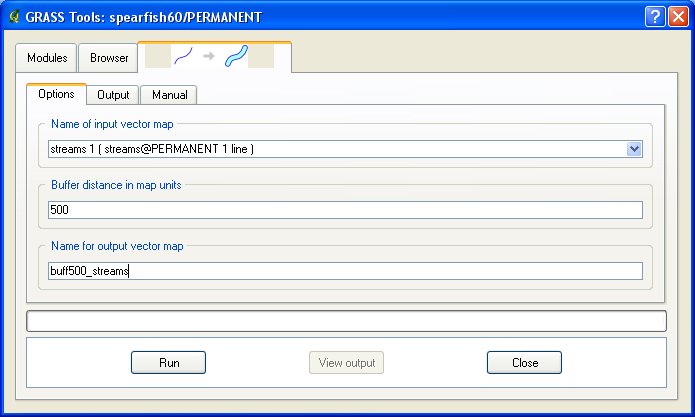
\includegraphics[scale=0.3]{qgis034.png}
   %caption of the figure
   \caption{}
   %label of the figure, which has to correspond to \ref{}:
   \label{fig:qgis034}
\end{figure}

Traitement de donn\'ees en cours... Fig.~\ref{fig:qgis035}

%\setkeys{Gin}{width=1\textwidth}
\begin{figure}[htbp]
   \centering
   %name of your graphic, without the path AND in PNG (screnshots etc)/PDF (drawings) format:
   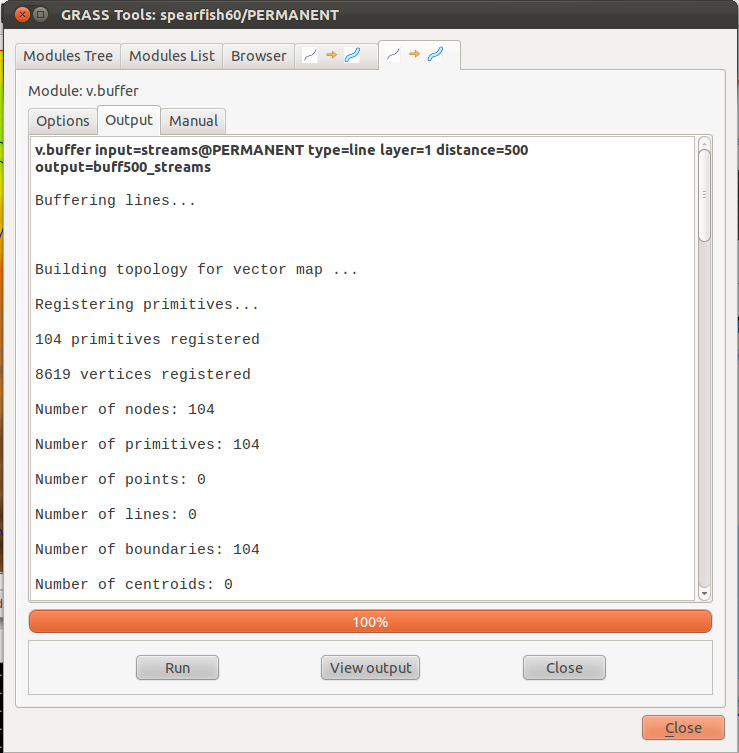
\includegraphics[scale=0.3]{qgis035.png}
   %caption of the figure
   \caption{}
   %label of the figure, which has to correspond to \ref{}:
   \label{fig:qgis035}
\end{figure}

Fin du traitement de donn\'ees Fig.~\ref{fig:qgis036}

%\setkeys{Gin}{width=1\textwidth}
\begin{figure}[htbp]
   \centering
   %name of your graphic, without the path AND in PNG (screnshots etc)/PDF (drawings) format:
   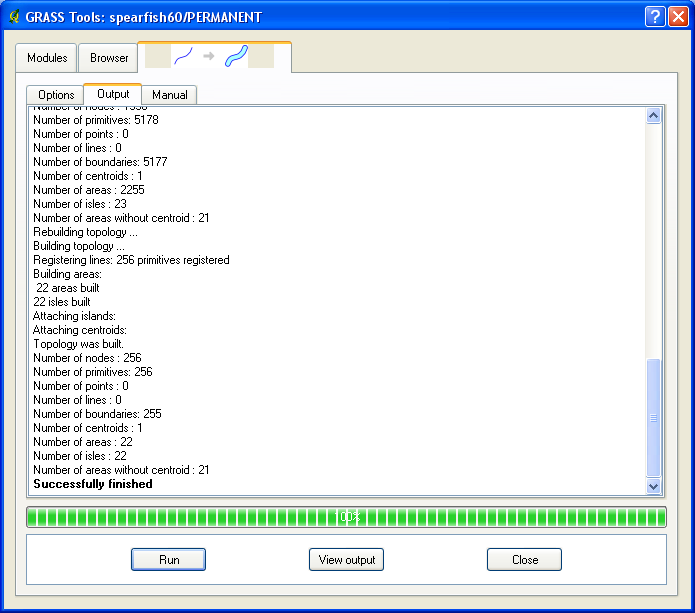
\includegraphics[scale=0.3]{qgis036.png}
   %caption of the figure
   \caption{}
   %label of the figure, which has to correspond to \ref{}:
   \label{fig:qgis036}
\end{figure}

Le r\'esultat devrait ressembler \`a cel\`a (Vous devrez charger la carte vous-m\^eme!) Fig.~\ref{fig:qgis037}

%\setkeys{Gin}{width=1\textwidth}
\begin{figure}[htbp]
   \centering
   %name of your graphic, without the path AND in PNG (screnshots etc)/PDF (drawings) format:
   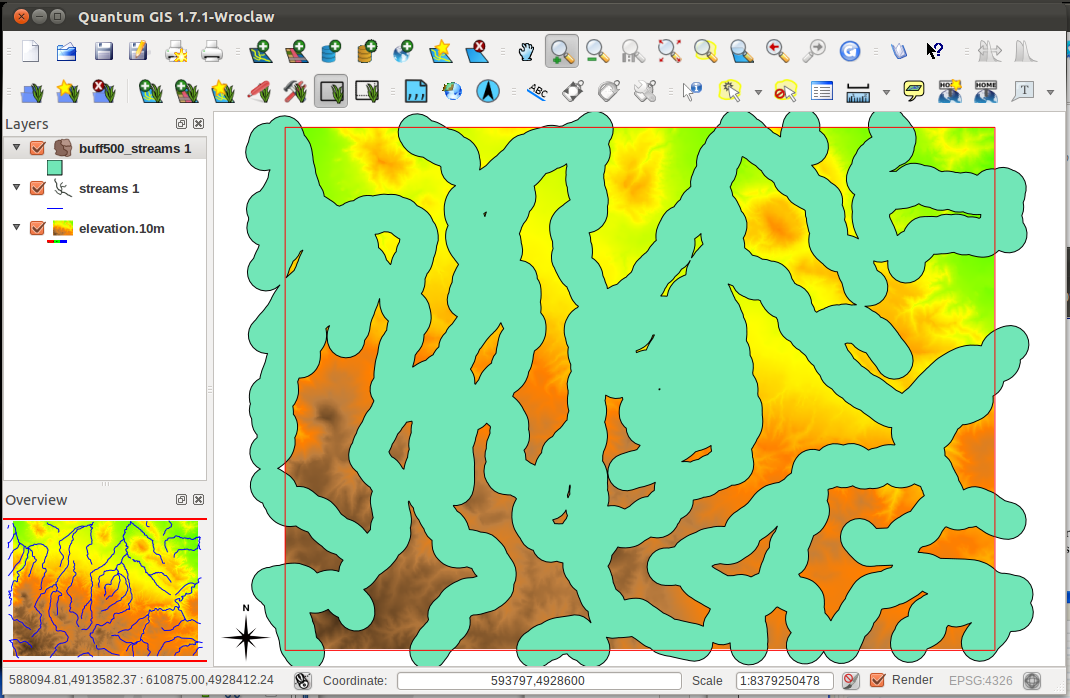
\includegraphics[scale=0.2]{qgis037.png}
   %caption of the figure
   \caption{}
   %label of the figure, which has to correspond to \ref{}:
   \label{fig:qgis037}
\end{figure}

Maintenant cr\'eez une autre zone tampon \`a partir de ``streams'' mais cette fois de 100 m\`etres... Comme ceci Fig.~\ref{fig:qgis038}

%\setkeys{Gin}{width=1\textwidth}
\begin{figure}[htbp]
   \centering
   %name of your graphic, without the path AND in PNG (screnshots etc)/PDF (drawings) format:
   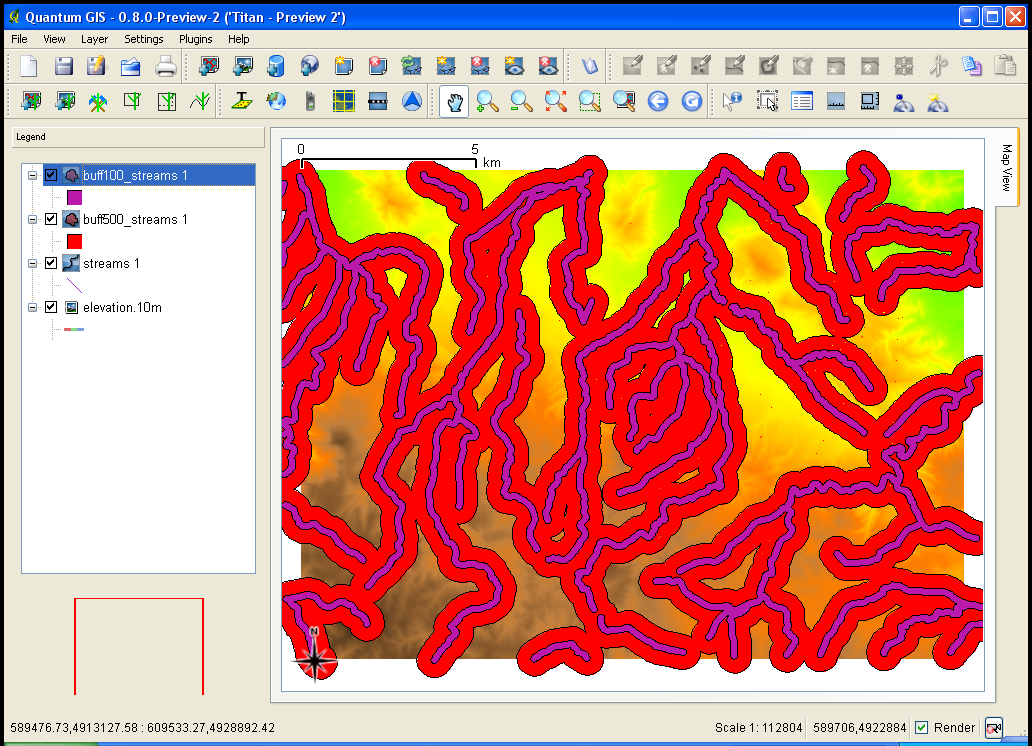
\includegraphics[scale=0.2]{qgis038.png}
   %caption of the figure
   \caption{}
   %label of the figure, which has to correspond to \ref{}:
   \label{fig:qgis038}
\end{figure}

Maintenant nous allons soustraire le buffer de 100m au buffer de 500m, car nous voulons exclure le cours d'eau et sa zone de proximit\'e de notre zone de s\'election. Trouvez ce module! Fig.~\ref{fig:qgis039}

%\setkeys{Gin}{width=1\textwidth}
\begin{figure}[htbp]
   \centering
   %name of your graphic, without the path AND in PNG (screnshots etc)/PDF (drawings) format:
   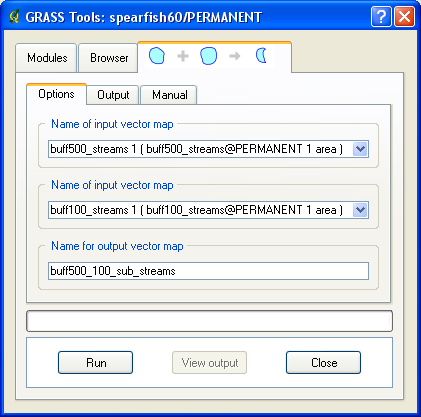
\includegraphics[scale=0.35]{qgis039.png}
   %caption of the figure
   \caption{}
   %label of the figure, which has to correspond to \ref{}:
   \label{fig:qgis039}
\end{figure}

Traitement de la superimposition de couches avec l'op\'erateur bool\'een ``NOT'' Fig.~\ref{fig:qgis040}

%\setkeys{Gin}{width=1\textwidth}
\begin{figure}[htbp]
   \centering
   %name of your graphic, without the path AND in PNG (screnshots etc)/PDF (drawings) format:
   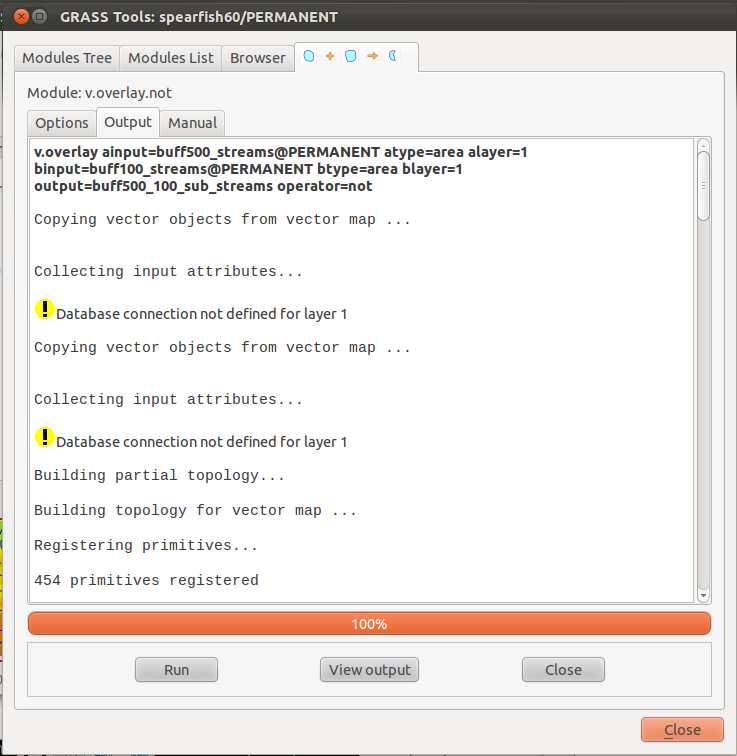
\includegraphics[scale=0.35]{qgis040.png}
   %caption of the figure
   \caption{}
   %label of the figure, which has to correspond to \ref{}:
   \label{fig:qgis040}
\end{figure}

Le r\'esultat est d'enlever tout dans les 100m des cours d'eau, et tout au-del\`a des 500m des cours d'eau. Fig.~\ref{fig:qgis041}

%\setkeys{Gin}{width=1\textwidth}
\begin{figure}[htbp]
   \centering
   %name of your graphic, without the path AND in PNG (screnshots etc)/PDF (drawings) format:
   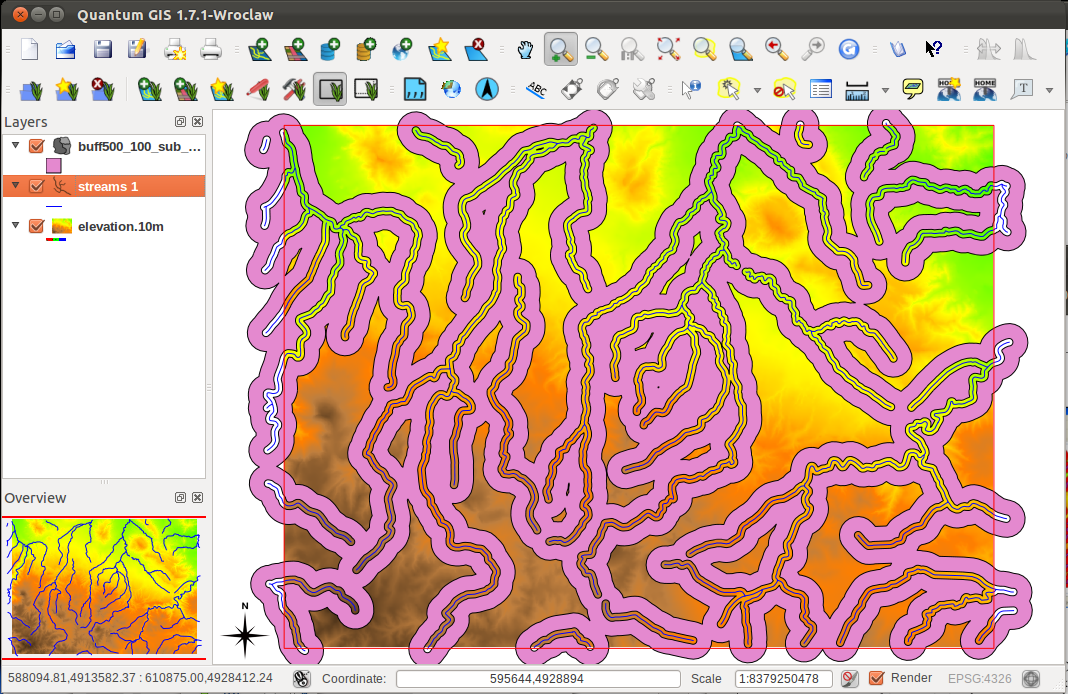
\includegraphics[scale=0.2]{qgis041.png}
   %caption of the figure
   \caption{}
   %label of the figure, which has to correspond to \ref{}:
   \label{fig:qgis041}
\end{figure}

Traitement d'un carte d'aspect \`a partir de la carte d'altitude Fig.~\ref{fig:qgis042}

%\setkeys{Gin}{width=1\textwidth}
\begin{figure}[htbp]
   \centering
   %name of your graphic, without the path AND in PNG (screnshots etc)/PDF (drawings) format:
   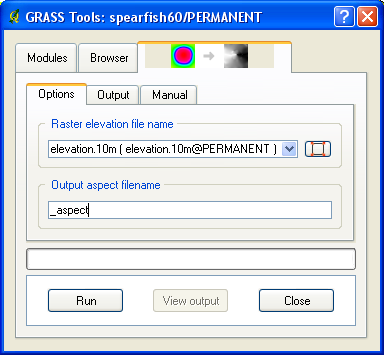
\includegraphics[scale=0.45]{qgis042.png}
   %caption of the figure
   \caption{}
   %label of the figure, which has to correspond to \ref{}:
   \label{fig:qgis042}
\end{figure}

Traitement en cours... Fig.~\ref{fig:qgis043}

%\setkeys{Gin}{width=1\textwidth}
\begin{figure}[htbp]
   \centering
   %name of your graphic, without the path AND in PNG (screnshots etc)/PDF (drawings) format:
   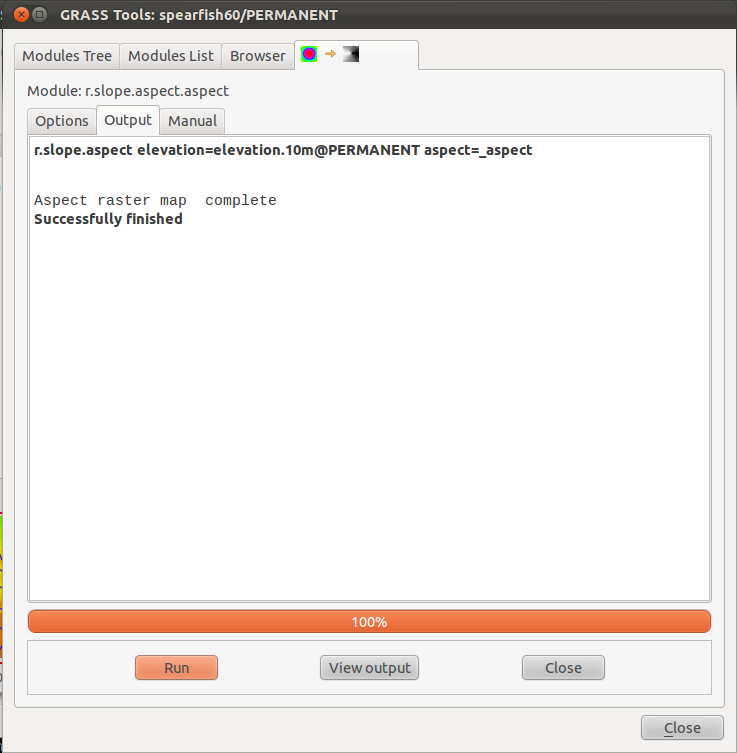
\includegraphics[scale=0.45]{qgis043.png}
   %caption of the figure
   \caption{}
   %label of the figure, which has to correspond to \ref{}:
   \label{fig:qgis043}
\end{figure}

Result Fig.~\ref{fig:qgis044}

%\setkeys{Gin}{width=1\textwidth}
\begin{figure}[htbp]
   \centering
   %name of your graphic, without the path AND in PNG (screnshots etc)/PDF (drawings) format:
   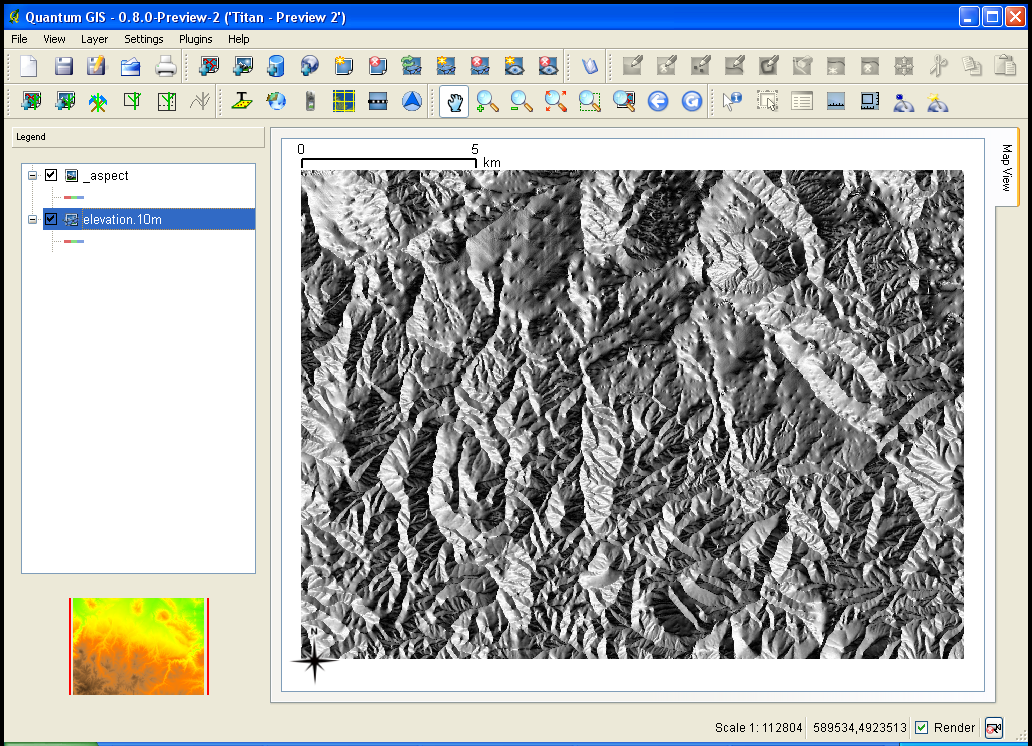
\includegraphics[scale=0.2]{qgis044.png}
   %caption of the figure
   \caption{}
   %label of the figure, which has to correspond to \ref{}:
   \label{fig:qgis044}
\end{figure}

\address{GRASS Development Team\\
  \url{http://grass.itc.it}\\
  \email{weblist@grass.itc.it}}

%%% Local Variables: 
%%% mode: latex
%%% TeX-master: main_document.tex
%%% End:

